\input{preamble}

\begin{document}

\pagestyle{fancy}
\fancyhead[L]{Seconde}
\fancyhead[C]{\textbf{TD n°3 : plan cartésien}}
\fancyhead[R]{\today}

Dans les exercices de ce TD, et sauf mention contraire explicite, 
\textbf{on supposera toujours que le plan cartésien est muni d'un repère orthonormé}.

\exe{}{
	Donner approximativement les coordonnées de chaque point du repère ci-contre.

	\begin{center}
	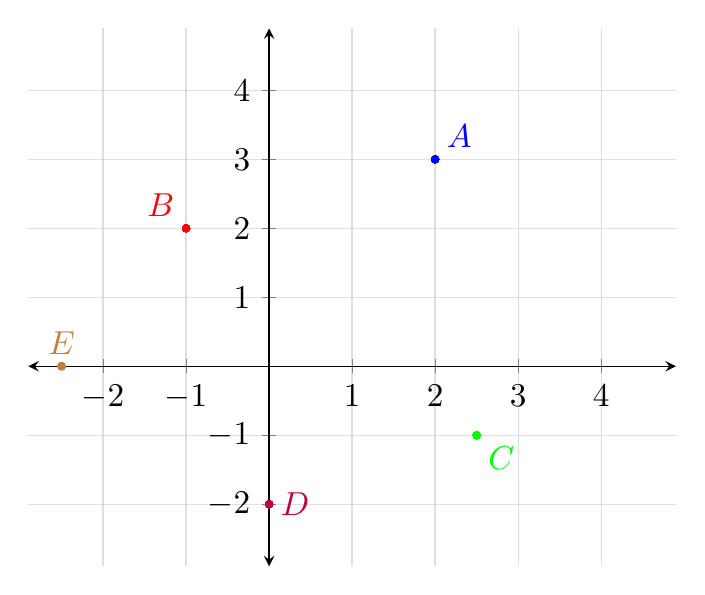
\begin{tikzpicture}[>=stealth, scale=1.2]
		\begin{axis}[xmin = -2.9, xmax=4.9, xtick={ -3, ..., 5}, ymin=-2.9, ymax=4.9, ytick={-3, ..., 5}, axis x line=middle, axis y line=middle, axis line style=<->, xlabel={}, ylabel={}, grid=both, grid style = {opacity=.5}]			
			\addplot[blue, mark=*, mark size = 1] (2,3) node[above right] {$A$};
			\addplot[red, mark=*, mark size = 1] (-1,2) node[above left] {$B$};
			\addplot[green, mark=*, mark size = 1] (2.5,-1) node[below right] {$C$};
			\addplot[purple, mark=*, mark size = 1] (0,-2) node[right] {$D$};
			\addplot[brown, mark=*, mark size = 1] (-2.5,0) node[above] {$E$};
		\end{axis}
	\end{tikzpicture}
	\end{center}
}{exe:1}{
	\begin{align*}
		A(2 ; 3) && B(-1 ; 2) && C(2,5 ; -1) &&
		D(0;-2) && E(-2,5 ; 0)
	\end{align*}
}

\exe{}{
En reprenant les points de l'exercice précédent calculer :
\begin{enumerate}
\item Les longueurs des segments $[AB]$ et $[BD]$.
\item Les coordonnées du point $M$, milieu du segment $[AD]$.
\end{enumerate}
}{exe:2}{
\begin{enumerate}
\item $AB = \sqrt{10}$ et $BD=\sqrt{17}$.
\item $M(1;1/2)$.
\end{enumerate}
}

\exe{}{
On considère les points $A(-5, 3)$ et $B(2,4)$ du plan cartésien. 
\begin{enumerate}
\item
Déterminer la longueur du segment $[AB]$.
\item
Déterminer les coordonnées du point $M$ milieu du segment [AB]. Quelle est la distance entre les points $B$ et $M$ ?
\end{enumerate}
}{exe:3}{
\begin{enumerate}
\item
$AB=\sqrt{50}$.
\item
$M(-3/2;1)$ et $BM=\sqrt{50}/2$.
\end{enumerate}
}

\exe{, difficulty=1}{
On place dans le plan cartésien les points $A(2,4), B(8,5)$ et $D(4,0)$. 
\begin{enumerate}
\item Déterminer les coordonnées du point $C$ pour que $ABCD$ soit un parallélogramme. 
\item Déterminer les coordonnées du point d'intersection des droites $(AC)$ et $(BD)$.
\end{enumerate}
\textit{Indication : faites un dessin !} 
}{exe:4}{
\begin{enumerate}
\item $C(10;1)$.
\item Les diagonales d'un parallélogramme se coupent en leur milieu donc, en notant I se point d'intersection $I(6; 5/2)$.
\end{enumerate}
}

\exe{}{
	Donner des points du plan cartésien (par leurs coordonnées) tels que, lorsque reliés adéquatement, 
	on puisse lire la première lettre de votre prénom.
}{exe:5}{
Je prétend que mon prénom est Lionel. Les points $A(1;2), B(1;1)$ et $C(2,1)$ conviennent.
}

\exe{, difficulty=1}{
	Soient $A$ et $B$ deux points du plan cartésien. Montrer que $AB = 0$ si et seulement si $A=B$.
}{exe:6}{
Supposons que $AB = 0$, notons $A(x_A ; y_A)$ et $B(x_B ; y_B)$ les coordonnées des points. On a :
\[ (x_A - x_B)^2 + (y_A - y_B)^2 = 0, \]
or, pour $x \in \R$, on a toujours $x^2 \geq 0$ et $x^2 = 0$ si, et seulement si $x=0$. Donc
\[ x_A - x_B = 0 \qquad \text{et} \qquad y_A - y_B, \]
ce qui revient à dire que $x_A=x_B$ et $y_A=y_B$. Les points $A$ et bien sont donc les mêmes. \\

Supposons maintenant que $A=B$, autrement dit les points ont les mêmes coordonnées. 
En calculant $AB$ avec la formule on trouve bien $AB=0$.
}

\exe{}{
	On considère le triangle de sommets $A(1;2), B(-3 ; 5), C(-5 ; -6)$.
	\begin{enumerate}
		\item Tracer le triangle $ABC$ dans un repère.
		\item Calculer le carré de chacun des côtés. 
		\item Que dire du triangle ?
	\end{enumerate}
}{exe:7}{
	\begin{multicols}{2}
	\begin{center}
	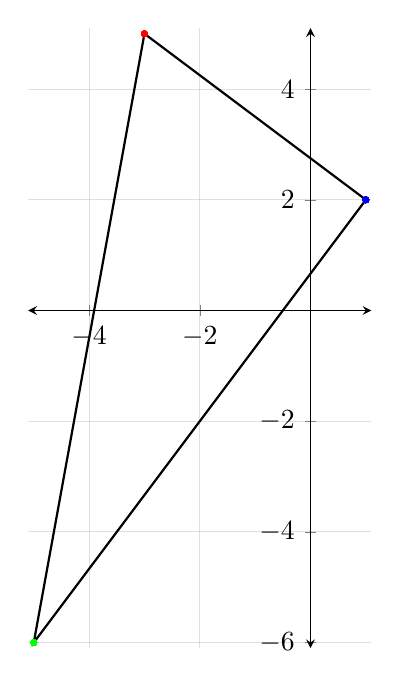
\begin{tikzpicture}[>=stealth, scale=1]
		\begin{axis}[xmin = -5.1, xmax=1.1, ymin=-6.1, ymax=5.1,axis x line=middle, axis y line=middle, axis line style=<->, xlabel={}, ylabel={}, grid=both, grid style = {opacity=.5}, x=20pt, y=20pt]			
			\addplot[blue, mark=*, mark size = 1] (1,2) node[above right] {$A$};
			\addplot[red, mark=*, mark size = 1] (-3,5) node[above left] {$B$};
			\addplot[green, mark=*, mark size = 1] (-5,-6) node[below right] {$C$};
			
			\draw[-, thick] (axis cs:1,2) -- (axis cs:-3,5) -- (axis cs:-5,-6) -- (axis cs:1,2);
		\end{axis}
	\end{tikzpicture}
	\end{center}
	
	\begin{enumerate}
		\item[2.] 
			\begin{align*}
				AB^2 & = 16 + 9 & = 25, \\
				AC^2 & = 36 + 64 & = 100, \\
				BC^2 &= 4 + 121 & = 125.
			\end{align*}
		\item[3.] D'après la réciproque du théorème de Pythagore, le triangle est rectangle en $A$ car $BC^2 = AB^2 + AC^2$.
	\end{enumerate}
	\end{multicols}
}

\newpage

\exe{, difficulty=2}{
On considère les point $A(5,2)$ et B$(1,-1)$ du plan cartésien et $\lambda$ un réel compris entre 0 et 1 : $0 \leq \lambda \leq 1$.
\begin{enumerate}
\item On considère le point $M$ de coordonnées 
\[ M(\lambda \cdot x_A + (1-\lambda) \cdot x_B, \lambda \cdot y_A + (1-\lambda) \cdot y_B), \]
placer les points $A, B$ et $M$ dans un repère orthonormé pour $\lambda = \frac12$. Que dire du point $M$ ?
\item On prend maintenant $\lambda = \frac13$. Placer le nouveau point $M$ (on le notera $M'$) dans un repère orthonormé.
\item Emettre un conjecture sur l'enemble des points 
\[ \{ M(\lambda \cdot x_A + (1-\lambda) \cdot x_B, \lambda \cdot y_A + (1-\lambda) \cdot y_B) \tq \lambda \in [0,1] \}. \]
\end{enumerate}
\textit{Indication : considérer les valeurs extrêmes de $\lambda$.}
}{exe:8}{
Solution non fournie, exercice de recherche.
}

\exe{, difficulty=2}{
On considère l'ensemble $C$ défini par 
\[ C = \{ (x,y) \tq x,y \in \R \text{ et } x^2 + y^2 = 1 \} . \]
\begin{enumerate}
\item Rappeler la définition du plan cartésien. En déduire que l'ensemble $C$ est inclus dans le plan cartésien.
\item On considère les points $(1,0), (0,1), (-1,0)$ et $(0,-1)$ du plan cartésien. Démontrer que ces points sont des éléments de $C$.
\item On suppose que le point $M(x_M, y_M)$ appartient à $C$. Calculer la distance entre l'origine $O$ du repère et $C$.
\item En déduire la nature géométrique de l'ensemble $C$.
\end{enumerate}
}{exe:9}{
Solution non fournie, exercice de recherche.
}

%%%%%%%%%%%%

\newpage
\fancyhead[C]{\textbf{Solutions}}
\shipoutAnswer

\end{document}
